% Sizes
\pgfmathsetmacro{\tilewidth}{6}
\pgfmathsetmacro{\tileheight}{6}
\pgfmathsetmacro{\supporttileheight}{0.5*\tileheight}
\pgfmathsetmacro{\tileMargin}{0.5}

\pgfmathsetmacro{\supportTileArrowWidth}{0.5*\tilewidth}

% Shapes
\tikzset{
	cardcorners/.style={
		rounded corners=0.2cm
	}
}
\tikzset{
	smallcardcorners/.style={
		rounded corners=0.1cm
	}
}


\def\shapeActionTile{(0,0) rectangle (\tilewidth,\tileheight)}
\def\shapeSupportActionTile{(0,0) rectangle (\tilewidth,\supporttileheight)}

\newcommand{\supportActionTile}[1]{
	\draw[lightgray,cardcorners,fill=gray] \shapeSupportActionTile;
	\draw[white,fill=white]
		(0.5*\tilewidth-0.5*\supportTileArrowWidth, \supporttileheight-\tileMargin) --
		(0.5*\tilewidth+0.5*\supportTileArrowWidth, \supporttileheight-\tileMargin) --
		(0.5*\tilewidth, \tileMargin) --
		cycle;
	\filldraw[red,fill=white!85!red] (0.5*\tilewidth+0.25*\supportTileArrowWidth, 0.5*\supporttileheight-\tileMargin) circle (0.5cm);
	\node[text width=0.5cm] at (0.5*\tilewidth+0.25*\supportTileArrowWidth, 0.5*\supporttileheight-0.5*\tileMargin) {
		\begin{center}
			#1
		\end{center}
	};
}

\newcommand{\actionTile}{
	\draw[lightgray,cardcorners] \shapeActionTile;
}

\newcommand{\actionTileCost}[1]{
	\filldraw[red,fill=white!85!red] (0.5*\tilewidth, 0.85*\tileheight) circle (0.5cm);
	\node[text width=0.5cm] at (0.5*\tilewidth, 0.85*\tileheight+0.5*\tileMargin) {
		\begin{center}
			#1
		\end{center}
	};
}
\newcommand{\terraformingReward}[1]{
	\filldraw[green,fill=white!85!green] (\tileMargin, \tileMargin) rectangle (\tilewidth-\tileMargin, \tileMargin+0.75);
	\node[text width=\tilewidth cm] at (0.5*\tilewidth, \tileMargin+0.5) {
		\begin{center}
			\raisebox{0.25cm}{#1}
			
\includegraphics[height=0.7cm]{icons/achievement_white.png}
		\end{center}
	};
}

\newcommand{\activateProjectsAction}{
	\node[text width=\tilewidth cm] at (0.5*\tilewidth, 0.5*\tileheight) {
		\begin{center}
			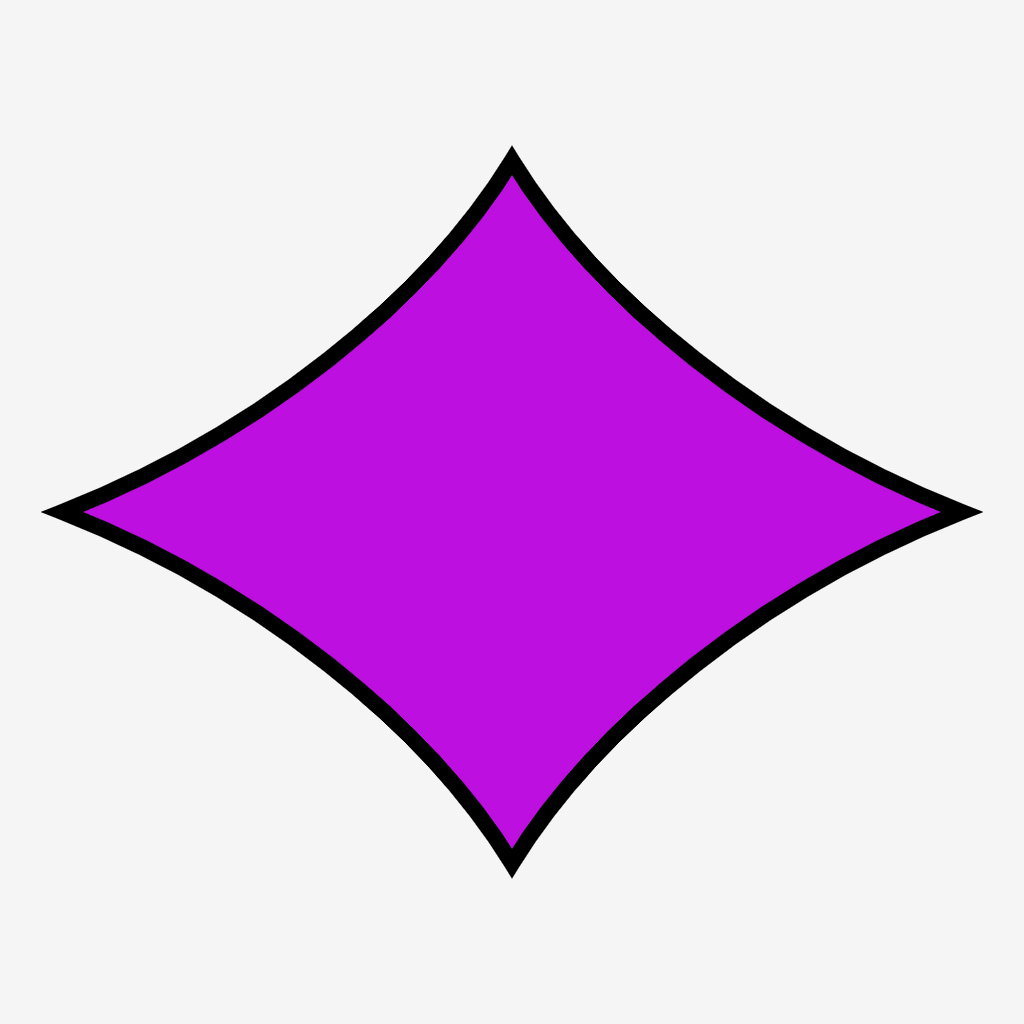
\includegraphics[width=1.5cm,height=3cm]{icons/activation_diamond_purple_189-16-224.png}
			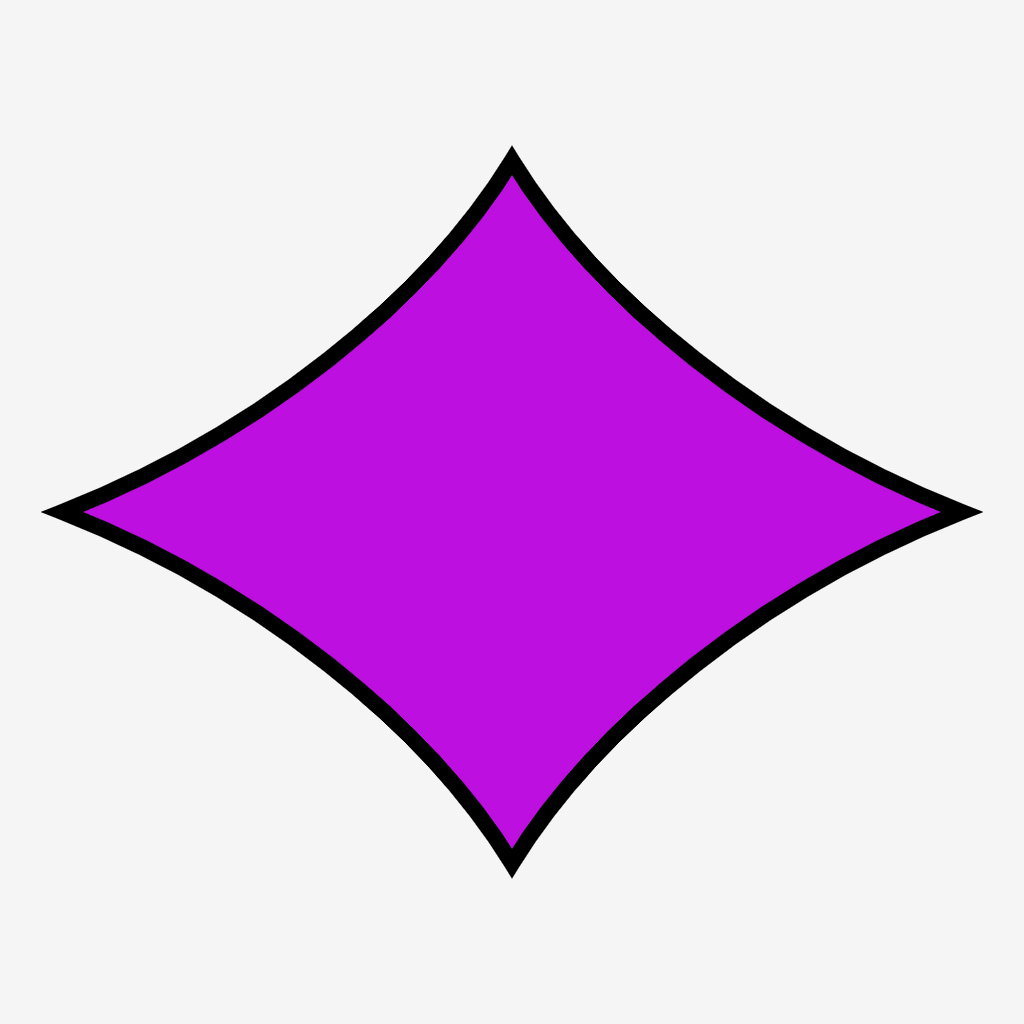
\includegraphics[width=1.5cm,height=3cm]{icons/activation_diamond_purple_189-16-224.png}
		\end{center}
	};
}

\newcommand{\groomProjectsAction}{
	\draw[black,smallcardcorners,fill=black] (\tileMargin,0.5*\tileheight-0.65) rectangle (0.33*\tilewidth-\tileMargin,0.5*\tileheight+0.65);
	\node[text width=2cm] at (0.33*\tilewidth, 0.5*\tileheight-0.5) {
		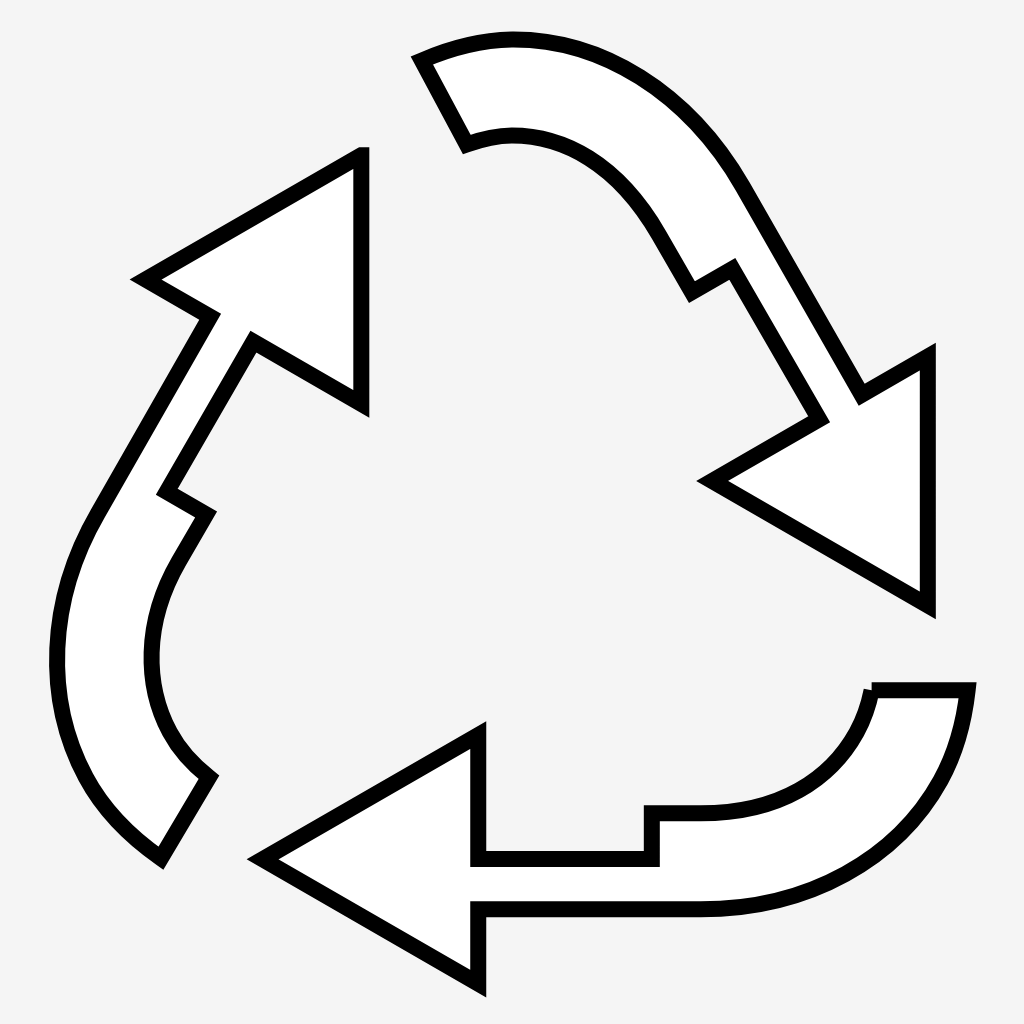
\includegraphics[width=0.75 cm]{icons/recycle.png}
	};
	\node[text width=2cm] at (0.5*\tilewidth, 0.5*\tileheight) {
		
\includegraphics[width=1.5 cm]{icons/card_draw.png}
	};
	\node[text width=2cm] at (0.85*\tilewidth, 0.5*\tileheight) {
		
\includegraphics[width=1.5 cm]{icons/card_draw.png}
	};
}

\newcommand{\implementProjectAction}{
	\draw[black,smallcardcorners,fill=black] (0.5*\tilewidth-1,0.5*\tileheight-1.5) rectangle (0.5*\tilewidth+1,0.5*\tileheight+1.5);
	\node[text width=2cm] at (0.5*\tilewidth, 0.5*\tileheight-1.25) {
		\begin{center}
			
\includegraphics[width=1.5 cm]{icons/play_arrow_white.png}
		\end{center}
	};
	\filldraw[red,fill=white!85!red] (0.5*\tilewidth+1, 0.5*\tileheight+1.5) circle (0.5cm);
	\node[text width=0.5cm] at (0.5*\tilewidth+1, 0.5*\tileheight+1.5+0.5*\tileMargin) {
		\begin{center}
			X
		\end{center}
	};
}

\newcommand{\placeForestAction}{
	\node[flathexa,fill=forest] at (0.5*\tilewidth, 0.5*\tileheight-0.5*\hexSize) {
		
\includegraphics[width=\hexIconSize cm]{icons/leaf_white.png}
	};
}

\newcommand{\placeWaterAction}{
	\node[flathexa,fill=water] at (0.5*\tilewidth, 0.5*\tileheight-0.5*\hexSize) {
		
\includegraphics[width=\hexIconSize cm]{icons/water_white.png}
	};
}

\newcommand{\placeCityAction}{
	\node[flathexa,fill=city] at (0.5*\tilewidth, 0.5*\tileheight-0.5*\hexSize) {
		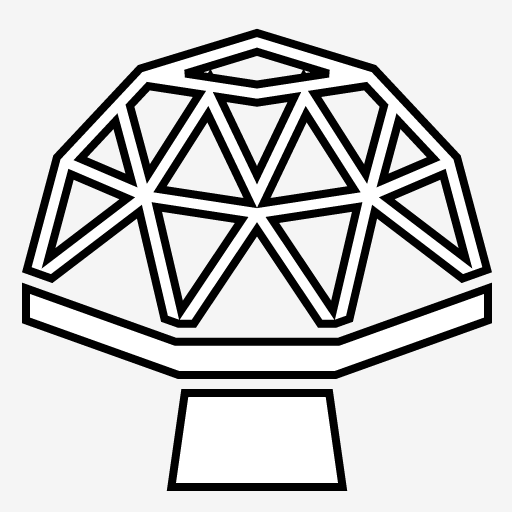
\includegraphics[width=\hexIconSize cm]{icons/city_white.png}
	};
}
